\documentclass[letterpaper, 11pt, openany]{book}
\usepackage[centertags]{amsmath}
\usepackage[pdflatex]{fullbib}
\usepackage{graphicx,amsfonts,amssymb,amsthm,newlfont,macros,referencing}
\usepackage{tikz}
\usepackage{float}
\usepackage{graphics}
\usepackage{caption}
\usepackage{booktabs}

\title{MTHE 332/393 Lab Manual (Solutions)}
\date{\today}
\sloppy
\begin{document}
\maketitle
%LAB1
\chapter{Intro}
\section{Deliverables}

\begin{enumerate}
\item Plots of motor position ($\theta$) and velocity ($\omega$) with respect to time
\item What is the steady state angular velocity (in rads/s) of the motor? 
Does this correlate to the vlaue obtained using the encoder plot?
\item Determine the motor constant $\tau$. Include a plot at t=$\tau$ (use proper units)
\item Determine the motor torque constant, $K_E$ (include units). Show your calculations.
\end{enumerate}

\section{Solutions}
\begin{enumerate}
\item 
The plots for position and angular velocity of the motor can be found in figures~\ref{fig:Theta},
~\ref{fig:Omega}. 
\begin{figure}[htbp]
\centering
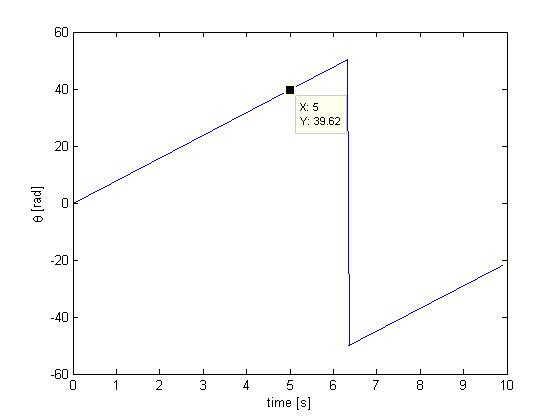
\includegraphics[width=0.9\textwidth, height = 7cm]{graphics/Theta_Lab1.jpg} 
\caption{Plot for theta vs time for Lab 1}\label{fig:Theta}
\end{figure}

\begin{figure}[htbp]
\centering
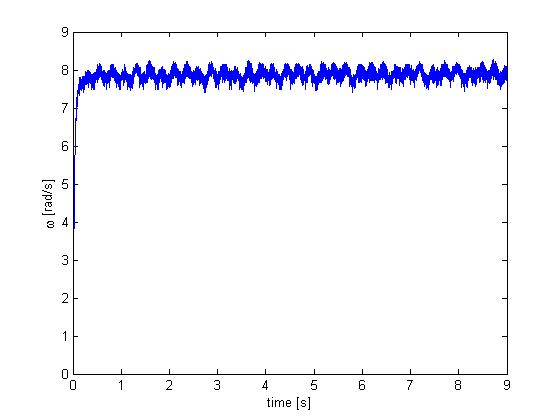
\includegraphics[width=0.9\textwidth, height = 7cm]{graphics/Omega_Lab1.jpg} 
\caption{Plot of omega vs time for Lab 1}\label{fig:Omega}
\end{figure}


\item Steady state angular velocity is roughly 8.25 rads/s

\item By manipulating the solution to equation %REFERENCE
The motor constant $\tau$ was found to be roughly 0.036. A 
zoomed in plot of the angular velocity at $t = \tau$ can be found in
figure~\ref{fig:Tau}

\begin{figure}[htbp]
\centering
\includegraphics[width=0.9\textwidth, height = 7cm]{graphics/t=Tau.jpg} 
\caption{Zoomed in plot of omega vs time at $t = \tau$}\label{fig:Tau}
\end{figure}

\item By using the value of $\tau$ and rearranging equation %REFERENCE,
$K_E$ was found to be 229.16. 
\end{enumerate}


%LAB2
\chapter{Frequency Response}
\section{Deliverables}

\begin{enumerate}
\item Include the Matlab generated bode plots for $\theta$ and $\omega$. Use your $K_E$ and $\tau$ values
from lab 1
\item Plots of your motor angular position and velocity and the input function $u =  5\sin(t^2).$ 
Comment on the general trend of the magnitude and phase shift of the outputs. Does this agree
with the bode plots you generated?
\item Include the tabulated data gathered from your experimental Bode plots. 
\item Include experimental bode plots for both magnitude and phase difference.
\end{enumerate}

\section{Solutions}
\begin{enumerate}
\item Figures~\ref{fig:BodeTheta} and~\ref{fig:BodeOmega} show the Matlab generated 
Bode plots for the systems angular position and velocity. 
\begin{figure}[htbp]
\centering
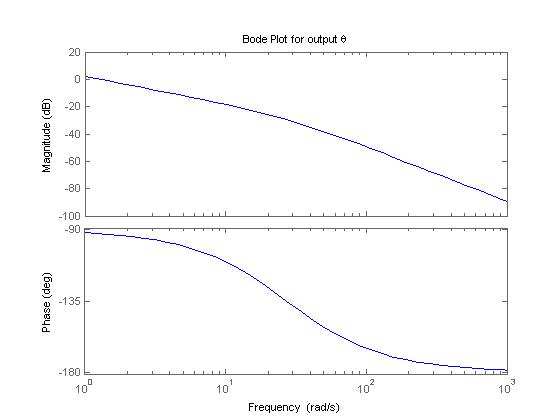
\includegraphics[width=0.9\textwidth, height = 7cm]{graphics/BodeTheta.jpg} 
\caption{Matlab generated Bode plot for output $\theta$}\label{fig:BodeTheta}
\end{figure}

\begin{figure}[htbp]
\centering
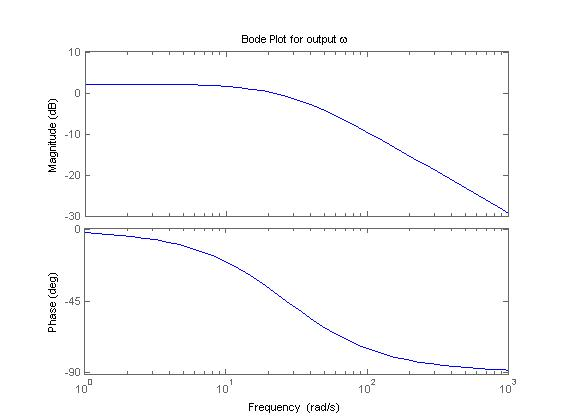
\includegraphics[width=0.9\textwidth, height = 7cm]{graphics/BodeOmega.jpg} 
\caption{Matlab generated Bode plot for output $\omega$}\label{fig:BodeOmega}
\end{figure}

\item Figures~\ref{fig:Thetatsquared} and~\ref{fig:Omegatsquared} show the systems response 
to an input of a harmonic signal with increasing frequency. As you can see, the magnitude of 
the output decreases as the frequency increases, which agrees with the Bode plot generated 
in Matlab.
\begin{figure}[htbp]
\centering
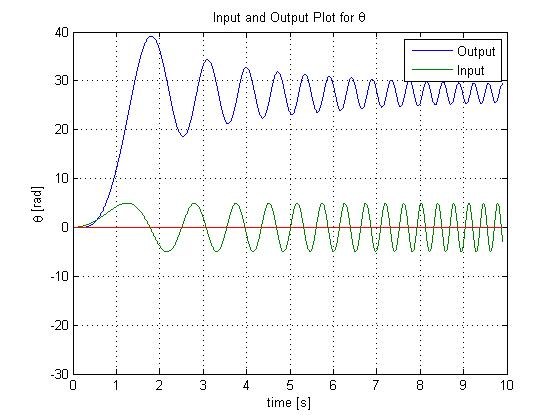
\includegraphics[width=0.9\textwidth, height = 7cm]{graphics/Thetatsquared.jpg} 
\caption{Input and output for $\theta$ for the input $5\sin(t^2)$}\label{fig:Thetatsquared}
\end{figure}

\begin{figure}[htbp]
\centering
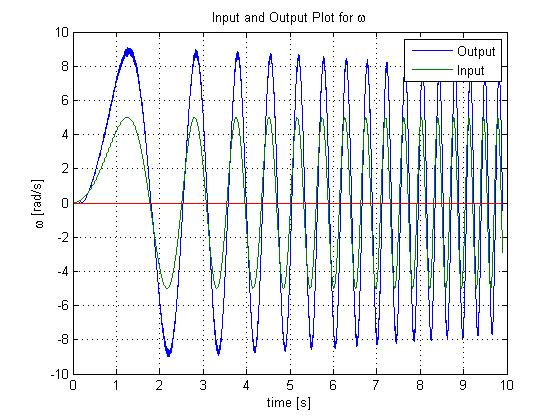
\includegraphics[width=0.9\textwidth, height = 7cm]{graphics/Omegatsquared.jpg} 
\caption{Input and output for $\omega$ for the input $5\sin(t^2)$}\label{fig:Omegatsquared}
\end{figure}

\item Table~\ref{tab:BodeData} includes data for the experimental Bode plots. 

\begin{table}[htbp]
  \centering
  \caption{Tabulated data  for experimental Bode plots. }
    \begin{tabular}{|r|r|r|r|r|r|}
    \toprule
    \multicolumn{1}{|p{3.28em}|}{\textbf{Omega (rad/s)}} & \multicolumn{1}{p{6.445em}|}{\textbf{Magnitude, M}} & \multicolumn{1}{p{4.28em}|}{\textbf{Gain (dB)}} & \multicolumn{1}{p{6.61em}|}{\textbf{Peak-time Diff (input-output)}} & \multicolumn{1}{p{5.11em}|}{\textbf{Phase (rad)}} & \multicolumn{1}{p{6.89em}|}{\textbf{Phase (degree)}} \\
    \midrule
    0.5   & 1.40  & 2.92  & 0     & 0     & 0.00 \\
    \midrule
    1     & 1.30  & 2.28  & 0     & 0     & 0.00 \\
    \midrule
    3     & 1.18  & 1.44  & 0     & 0     & 0.00 \\
    \midrule
    5     & 1.17  & 1.36  & 0     & 0     & 0.00 \\
    \midrule
    10    & 1.16  & 1.29  & -0.01 & -0.1  & -5.73 \\
    \midrule
    20    & 1.05  & 0.42  & -0.018 & -0.36 & -20.63 \\
    \midrule
    30    & 0.87  & -1.26 & -0.014 & -0.42 & -24.06 \\
    \midrule
    60    & 0.65  & -3.74 & -0.012 & -0.72 & -41.25 \\
    \midrule
    80    & 0.53  & -5.60 & -0.012 & -0.96 & -55.00 \\
    \midrule
    100   & 0.42  & -7.54 & -0.01 & -1    & -57.30 \\
    \midrule
    150   & 0.33  & -9.76 & -0.009 & -1.35 & -77.35 \\
    \midrule
    200   & 0.28  & -11.06 & -0.008 & -1.6  & -91.67 \\
    \midrule
    300   & 0.22  & -13.15 & -0.006 & -1.8  & -103.13 \\
    \bottomrule
    \end{tabular}%
  \label{tab:BodeData}%
\end{table}%



\item Figures~\ref{fig:MagBode} and~\ref{fig:PhaseBode} show the experimental 
bode plots for magnitude and phase difference when the output is $\omega$
\begin{figure}[htbp]
\centering
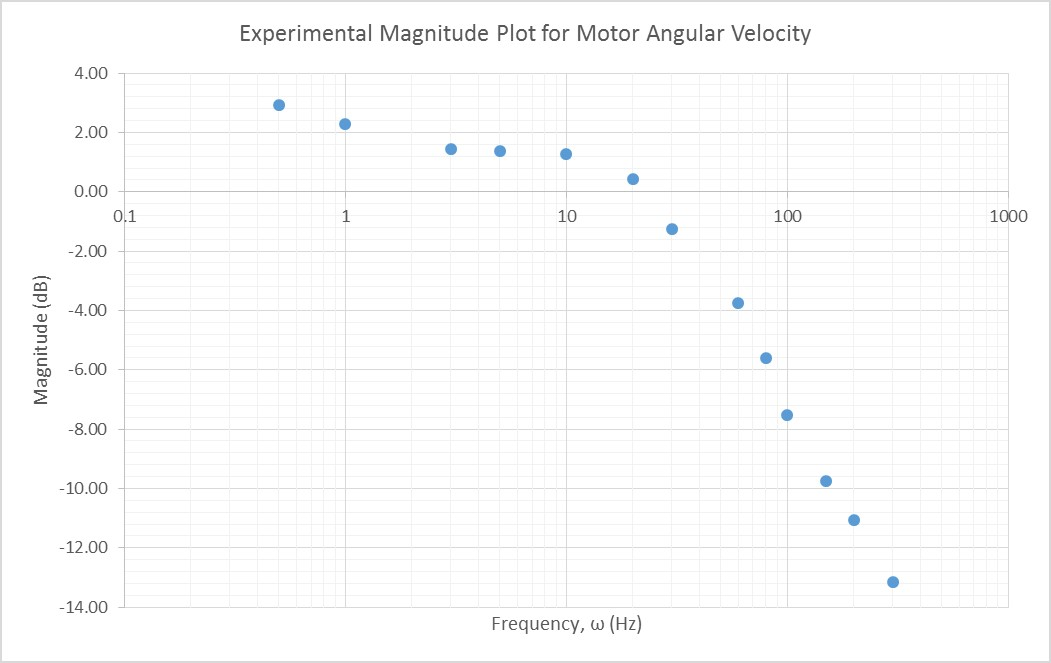
\includegraphics[width=0.9\textwidth, height = 7cm]{graphics/MagBode.jpg} 
\caption{Experimental magnitude Bode plot for $\omega$}\label{fig:MagBode}
\end{figure}

\begin{figure}[htbp]
\centering
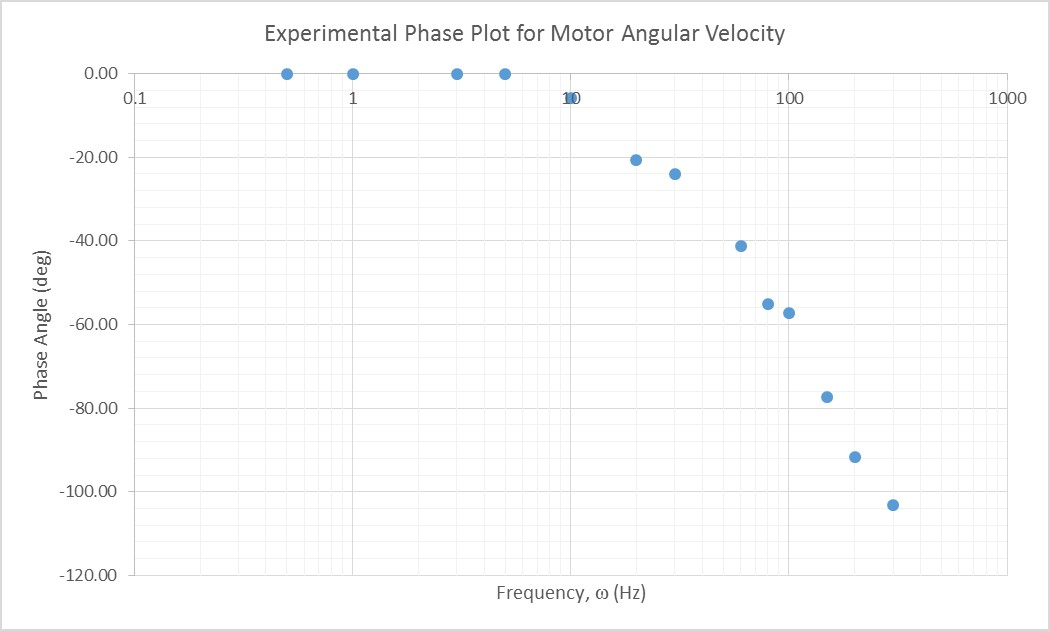
\includegraphics[width=0.9\textwidth, height = 7cm]{graphics/PhaseBode.jpg} 
\caption{Experimental phase Bode Plot for $\omega$}\label{fig:PhaseBode}
\end{figure}

\end{enumerate}

%LAB3
\chapter{PID}
\section{Deliverables}

\begin{enumerate}
\item Pick a good $K$ value (without P or D values), comment on how different values of $K$ affects overshoot,
 rise time, settling time, and steady state error. Note that a ``good" $K$ value is subjective, i.e. do you want
the system to respond quickly at the expense of accuracy, or slowly but extremely precisely? Justify your decision.
\item Include tabulated data of the response characteristics from steps~\ref{step:3},~\ref{step:4}, and~\ref{step:5}. 
\item Include the plot of the output that oscillates consistently about the reference trajectory of 10 radians 
generated in step~\ref{step:3}. Why does higher $K$ values increase the oscillation of the output? What is 
happening to the location of the closed loop poles? 
\item Include the plot of the output when using only integral control. Using the transfer function, determine the roots
of the characteristic polynomial.  What does this tell you about the behaviour of a system using only integral control?
\item Include a plot of the output using your PID controller when the desired angle is generated by the multi-input 
switch. Be sure to specify your P, I, and D values. 
\end{enumerate}

\section{Solutions}
\begin{enumerate}
\item For increasing $K$ values, overshoot and settling time will increase, but rise time and steady state error 
decreased.
\item Tables~\ref{tab:K_P},~\ref{tab:K_D}, and~\ref{tab:K_I} contain numerical values for rise time, 
settling time, overshoot, and steady state error for various values of $K_P$, $K_I$, and $K_D$.

% Table generated by Excel2LaTeX from sheet 'Sheet2'
\begin{table}[htbp]
  \centering
  \caption{Response characteristics for various $K_P$ with $K_I = 0, K_D = 0$}
    \begin{tabular}{rrrrr}
    \multicolumn{1}{l}{\textbf{K\_P}} & \multicolumn{1}{l}{\textbf{Overshoot}} & \multicolumn{1}{l}{\textbf{Rise Time}} & \multicolumn{1}{l}{\textbf{Settling Time}} & \multicolumn{1}{l}{\textbf{S.S. Error}} \\
    2     & 0.5   & 0.214 & 0.374 & 0.06 \\
    5     & 1.07  & 0.188 & 0.39  & 0.03 \\
    20    & 1.08  & 0.172 & 0.614 & 0.005 \\
    \end{tabular}%
  \label{tab:K_P}%
\end{table}%

% Table generated by Excel2LaTeX from sheet 'Sheet2'
\begin{table}[htbp]
  \centering
  \caption{Response characteristics for various $K_D$ with $K_P = 5, K_I = 0$}
    \begin{tabular}{rrrrr}
    \multicolumn{1}{l}{\textbf{K\_D}} & \multicolumn{1}{l}{\textbf{Overshoot}} & \multicolumn{1}{l}{\textbf{Rise Time}} & \multicolumn{1}{l}{\textbf{Settling Time}} & \multicolumn{1}{l}{\textbf{S.S. Error}} \\
    0.75  & 0     & 1.702 & 1.702 & 0.06 \\
    0.5   & 0     & 1.1   & 1.1   & 0.04 \\
    0.25  & 0     & 0.752 & 0.75  & 0.034 \\
    0.05  & 0.27  & 0.182 & 0.27  & 0.01 \\
    \end{tabular}%
  \label{tab:K_D}%
\end{table}%

% Table generated by Excel2LaTeX from sheet 'Sheet2'
\begin{table}[htbp]
  \centering
  \caption{Response characteristics for various $K_I$ with $K_P = 5, K_D = 0.25$}
    \begin{tabular}{rrrrr}
    \multicolumn{1}{l}{\textbf{K\_I}} & \multicolumn{1}{l}{\textbf{Overshoot}} & \multicolumn{1}{l}{\textbf{Rise Time}} & \multicolumn{1}{l}{\textbf{Settling Time}} & \multicolumn{1}{l}{\textbf{S.S. Error}} \\
    1     & 0.17  & 0.62  & \multicolumn{1}{l}{>10} & \multicolumn{1}{l}{?} \\
    0.75  & 0.11  & 0.8   & \multicolumn{1}{l}{>10} & \multicolumn{1}{l}{?} \\
    0.005 & 0     & 0.69  & 0.69  & 0.038 \\
    0.001 & 0     & 0.684 & 0.684 & 0.046 \\
    0.0005 & 0     & 0.666 & 0.666 & 0.034 \\
    \end{tabular}%
  \label{tab:K_I}%
\end{table}%


\item Figure~\ref{fig:Oscillate} demonstrates how significantly increasing the proportional control term 
can cause the system to oscillate about its reference trajectory. This is because increasing the $K$ value 
moves the poles of the closed loop transfer funciton closer to the imaginary axis.
 
\begin{figure}[htbp]
\centering
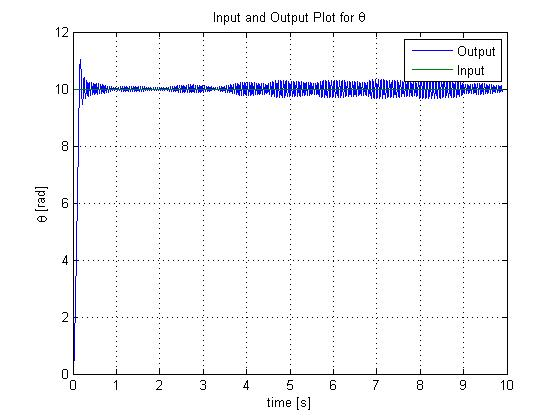
\includegraphics[width=0.9\textwidth, height = 7cm]{graphics/Oscillate.jpg} 
\caption{Input of 10 rads, K = 50, I = 0, D = 0}\label{fig:Oscillate}
\end{figure}
 
 \item Using only integral control puts a pole in the right half of the complex plane, making it no longer 
 BIBO stable. Therefore, the system can never be controlled by only integral control. Figure~\ref{fig:Integral}
 demonstrates this property.  
\begin{figure}[htbp]
\centering
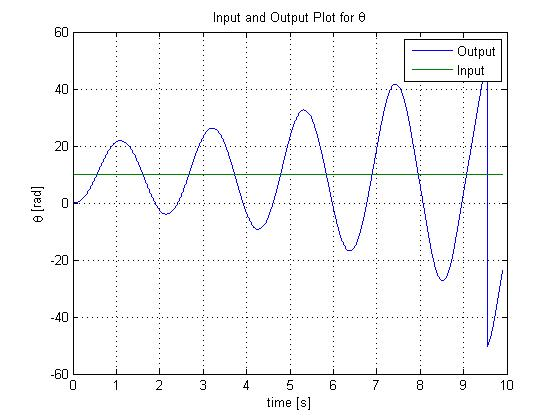
\includegraphics[width=0.9\textwidth, height = 7cm]{graphics/Integral.jpg} 
\caption{Input of 10 rads, K = 0, I = 1, D = 0}\label{fig:Integral}
\end{figure}
 
\item Figure~\ref{fig:Multiport} uses a PID controller with the optimal values for $K_P$, $K_I$, 
and $K_D$, and the reference trajectory is generated by the \verb|Multiport Switch| in Simulink. 
 
\begin{figure}[htbp]
\centering
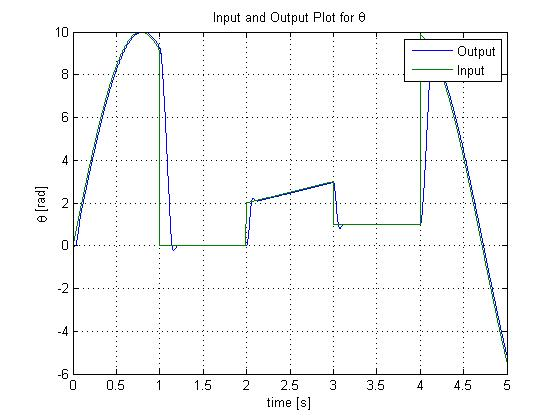
\includegraphics[width=0.9\textwidth, height = 7cm]{graphics/Multiport.jpg} 
\caption{Input and output of the system for a square wave function, with $K_P = 7$, $K_I = \frac{1}{125}$, and $K_D = \frac{1}{93}$}\label{fig:Multiport}
\end{figure}

\end{enumerate} 
 
 
%LAB4
\chapter{Performance Specs}
\section{Deliverables}

\begin{enumerate}
\item Include plots of the systems response with varying $\zeta$ and $\omega_0$ values, comment 
on the effect off varying these constants. 
\item For both positive and negative $\alpha$ values, what is the effect of increasing the magnitude 
of $\alpha$ on the rise time, settling time, overshoot/undershoot, and peak time? Include plots. 
\item Create the following table for the system type section. Be sure to include and reference all 
necessary plots for the justification section. 
\begin{table}[htbp]\label{tab:systype}
\centering
\begin{tabular}{|c|p{2.5cm}|p{2.5cm}|p{2.5cm}|c|c|}\hline
System No.&Response to Constant Input&Response to Ramp Input&Response to Quadratic Input&
Type?&Justification\\\hline
System 1&&&&&\\\hline
System 2&&&&&\\\hline
System 3&&&&&\\
\hline
\end{tabular}
\end{table}
\end{enumerate}


\section{Solutions}
\begin{enumerate}
\item Figure~\ref{fig:VaryOmega} shows the  step response of the system with varying values 
of $\omega_0$. It is clear that as $\omega_0$ increases, rise time, peak time, and settling time 
all decrease, but the overshoot remains constant. \\
Similarly, as $\zeta$ increases, both overshoot and settling time decrease, but rise time and 
peak time both increase. This can be seen in Figure~\ref{fig:VaryZeta}. 


\begin{figure}[htbp]
\centering
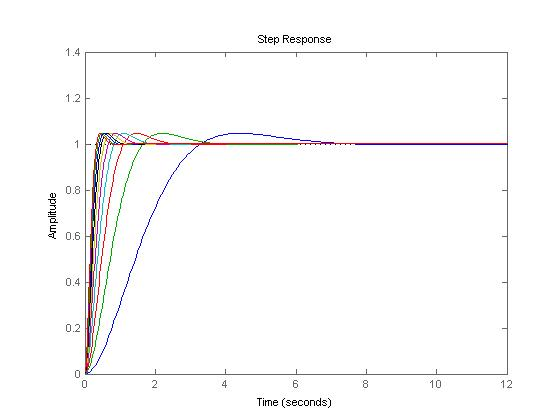
\includegraphics[width=0.9\textwidth, height = 7cm]{graphics/VaryOmega.jpg} 
\caption{Step response and impulse response of the system for $1 \leq \omega_0 \leq 10, \zeta = 0.7$}\label{fig:VaryOmega}
\end{figure}

\begin{figure}[htbp]
\centering
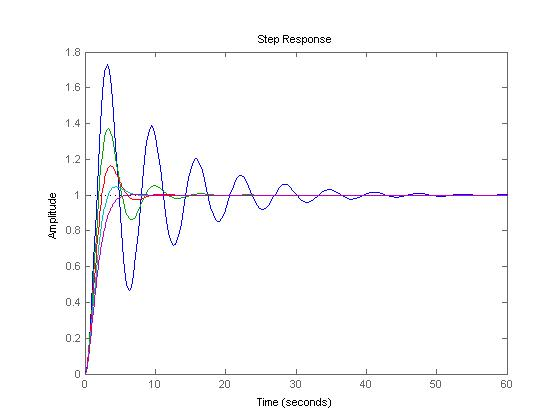
\includegraphics[width=0.9\textwidth, height = 7cm]{graphics/VaryZeta.jpg} 
\caption{Step response and impulse response of the system for $0.1 \leq \zeta \leq 0.9, \omega_0 = 1$}\label{fig:VaryZeta}
\end{figure}

\item Figure~\ref{fig:VaryAlphaPos} shows the effect of adding a zero ($\alpha$) to the systems transfer function. 
In this case, $\alpha$ varies from 1 to 9. As you can see, for positive values of $\alpha$, increasing the magnitude 
increases rise time and peak time, while settling time and overshoot decrease. Similarly for negative $\alpha$ shown 
in~\ref{fig:VaryAlphaNeg}, increasing the magnitude reduces overshoot, rise time, settling time, and peak time. 
Furthermore, adding a negative zero creates what is called undershoot, and the closer $\alpha$ is to the imaginary 
axis, the larger the undershoot becomes. 

\begin{figure}[htbp]
\centering
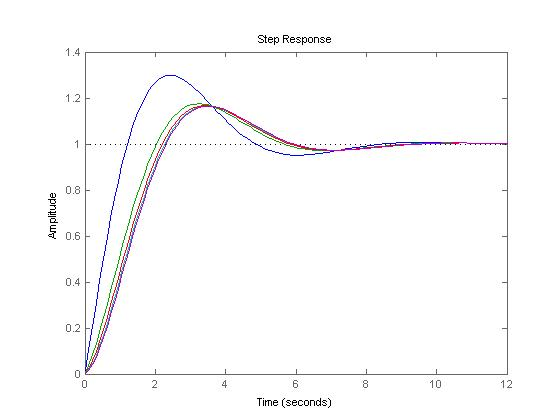
\includegraphics[width=0.9\textwidth, height = 7cm]{graphics/VaryAlphaPos.jpg} 
\caption{Step response and impulse response of the system with added zero ($1 \leq \alpha \leq 9$)}\label{fig:VaryAlphaPos}
\end{figure}

\begin{figure}[htbp]
\centering
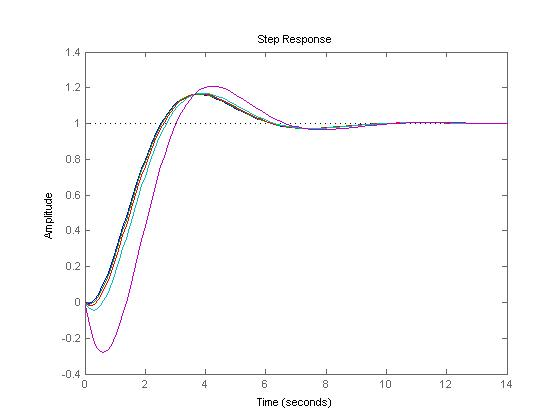
\includegraphics[width=0.9\textwidth, height = 7cm]{graphics/VaryAlphaNeg.jpg} 
\caption{Step response and impulse response of the system with added zero ($-9 \leq \alpha \leq -1$)}\label{fig:VaryAlphaNeg}
\end{figure}

\item Figures~\ref{fig:Const1}-~\ref{fig:Quad3Err} are plots of the systems response and error signal for 3 
different controllers (proportional, integral, and derivative) with 3 different inputs (constant, ramp, and quadratic). 
\begin{enumerate}
\item System 1: For this system, the error is bounded on a constant input, however it is unbounded for any polynomial 
with degree greater than 1. Therefore this system is type 1. \\

\begin{figure}[htbp]%System 1 Const
\centering
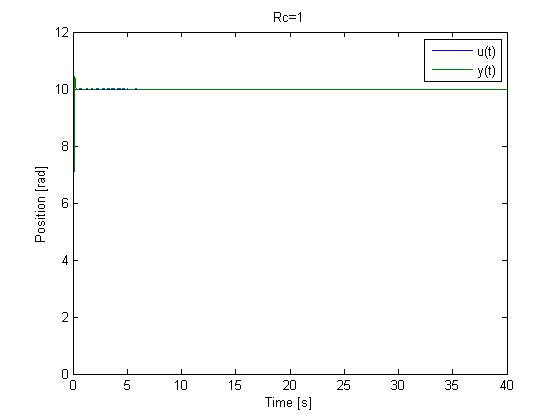
\includegraphics[width=0.9\textwidth, height = 7cm]{graphics/Const1.jpg} 
\caption{Systems response to constant input with $Rc = 1$}\label{fig:Const1}
\end{figure}

\begin{figure}[htbp]%System 1 Conts Error
\centering
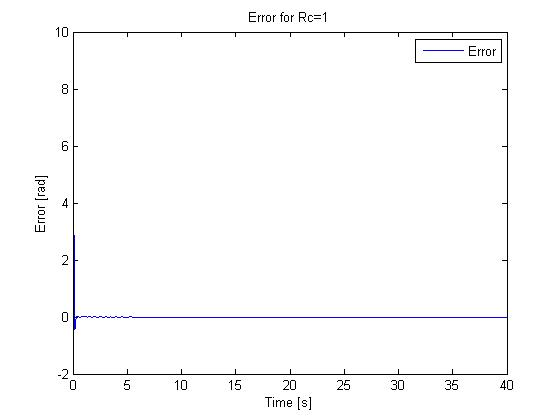
\includegraphics[width=0.9\textwidth, height = 7cm]{graphics/Const1Err.jpg} 
\caption{Systems error signal for constant input with $Rc = 1$}\label{fig:Const1Err}
\end{figure}

\begin{figure}[htbp]%System 1 Ramp
\centering
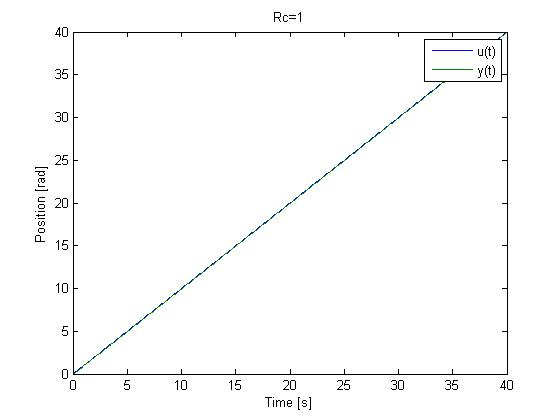
\includegraphics[width=0.9\textwidth, height = 7cm]{graphics/Ramp1.jpg} 
\caption{Systems response to a ramp input with $Rc = 1$}\label{fig:Ramp1}
\end{figure}

\begin{figure}[htbp]%System 1 Ramp Error
\centering
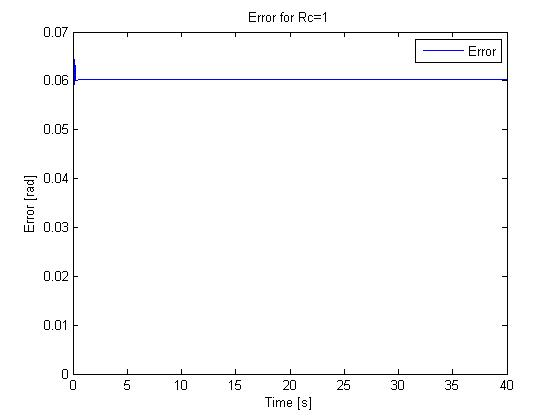
\includegraphics[width=0.9\textwidth, height = 7cm]{graphics/Ramp1Err.jpg} 
\caption{Systems error signal for a ramp input with $Rc = 1$}\label{fig:Ramp1Err}
\end{figure}

\begin{figure}[htbp]%System 1 Quadratic 
\centering
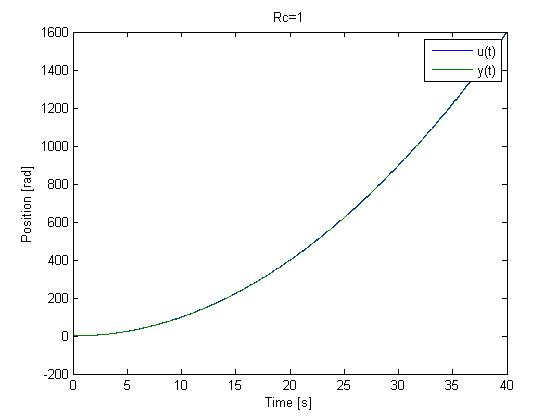
\includegraphics[width=0.9\textwidth, height = 7cm]{graphics/Quad1.jpg} 
\caption{Systems response to quadratic input with $Rc = 1$}\label{fig:Quad1}
\end{figure}

\begin{figure}[htbp]%System 1 Quad Error
\centering
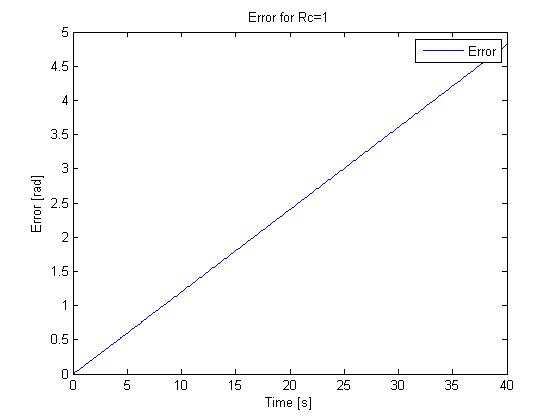
\includegraphics[width=0.9\textwidth, height = 7cm]{graphics/Quad1Err.jpg} 
\caption{Systems error signal for quadratic input with $Rc = 1$}\label{fig:Quad1Err}
\end{figure}

\item System 2: This system is type 0 because every input had unbounded error. \\
\begin{figure}[htbp]%System 2 Const
\centering
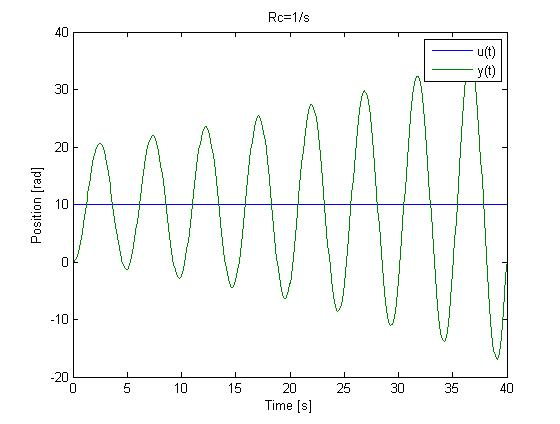
\includegraphics[width=0.9\textwidth, height = 7cm]{graphics/Const2.jpg} 
\caption{Systems response to constant input with $R_c = \frac{1}{s}$}\label{fig:Const2}
\end{figure}

\begin{figure}[htbp]%System 2 Const Err
\centering
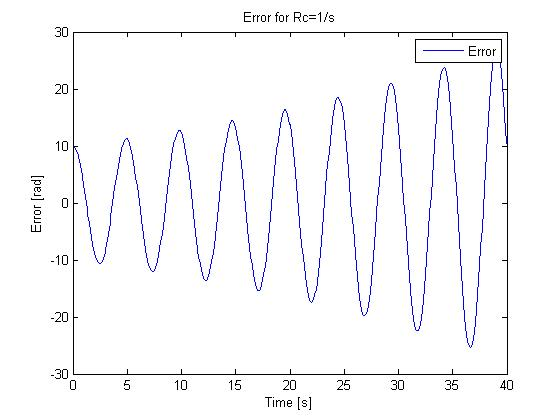
\includegraphics[width=0.9\textwidth, height = 7cm]{graphics/Const2Err.jpg} 
\caption{Systems error signal for constant input with $R_c = \frac{1}{s}$}\label{fig:Const2Err}
\end{figure}

\begin{figure}[htbp]%System 2 Ramp
\centering
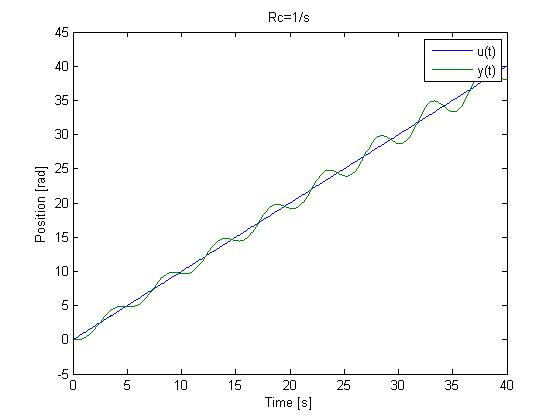
\includegraphics[width=0.9\textwidth, height = 7cm]{graphics/Ramp2.jpg} 
\caption{Systems response to a ramp input with $R_c = \frac{1}{s}$}\label{fig:Ramp2}
\end{figure}

\begin{figure}[htbp]%System 2 Ramp Err
\centering
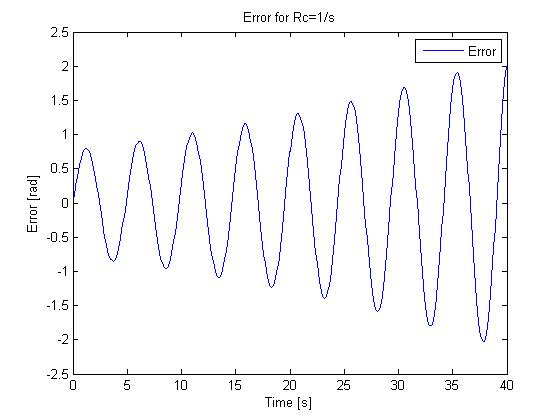
\includegraphics[width=0.9\textwidth, height = 7cm]{graphics/Ramp2Err.jpg} 
\caption{Systems error signal for a ramp input with $R_c = \frac{1}{s}$}\label{fig:Ramp2Err}
\end{figure}

\begin{figure}[htbp]%System 2 Quad
\centering
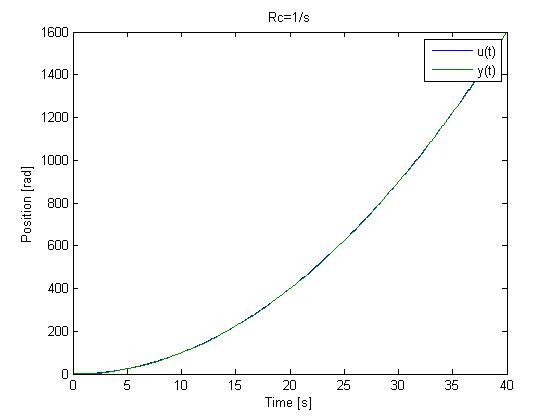
\includegraphics[width=0.9\textwidth, height = 7cm]{graphics/Quad2.jpg} 
\caption{Systems response to quadratic input with $R_c = \frac{1}{s}$}\label{fig:Quad2}
\end{figure}

\begin{figure}[htbp]%System 2 Quad Err
\centering
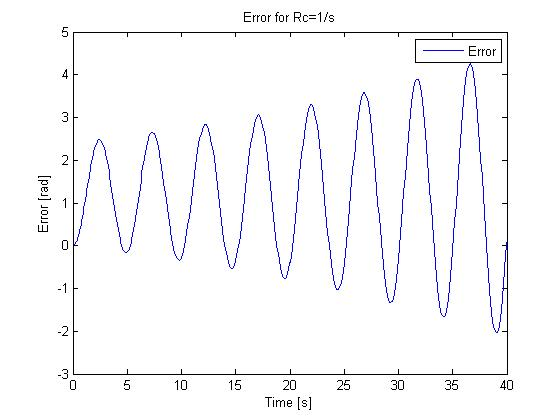
\includegraphics[width=0.9\textwidth, height = 7cm]{graphics/Quad2Err.jpg} 
\caption{Systems error signal for a quadratic input with $R_c = \frac{1}{s}$}\label{fig:Quad2Err}
\end{figure}

\item System 3: Lastly, this system is type 2, because the constant and ramp inputs had bounded error, and only the 
quadratic input had unbounded error. \\
\begin{figure}[htbp]%System 3 Const
\centering
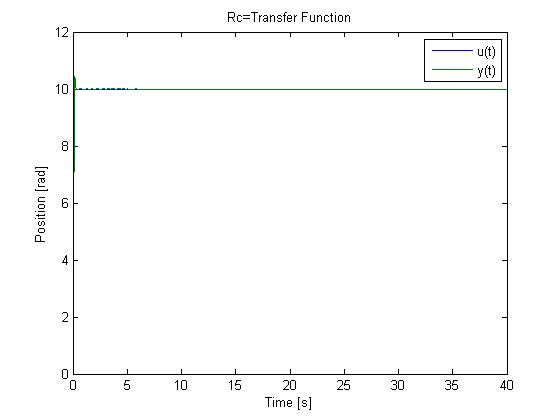
\includegraphics[width=0.9\textwidth, height = 7cm]{graphics/Const3.jpg} 
\caption{Systems response for a constant input with $R_c = s$}\label{fig:Const3}
\end{figure}

\begin{figure}[htbp]%System 3 Const Err
\centering
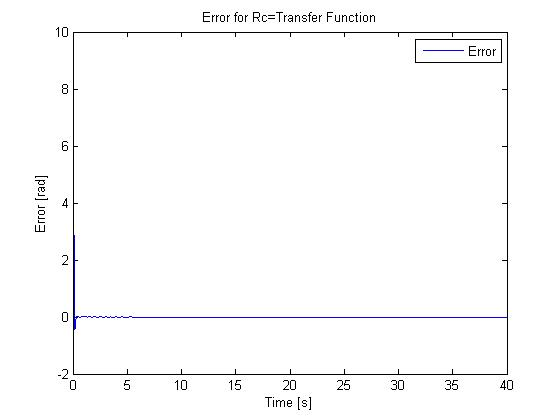
\includegraphics[width=0.9\textwidth, height = 7cm]{graphics/Const3Err.jpg} 
\caption{Systems error signal for for constant input with $R_c = s$}\label{fig:Const3Err}
\end{figure}

\begin{figure}[htbp]%System 3 Ramp
\centering
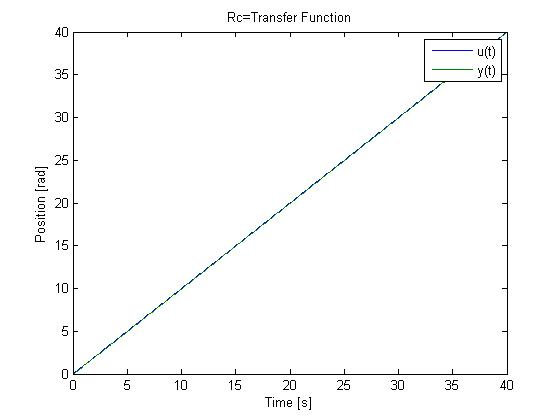
\includegraphics[width=0.9\textwidth, height = 7cm]{graphics/Ramp3.jpg} 
\caption{Systems response for a ramp input with $R_c = s$}\label{fig:Ramp3}
\end{figure}

\begin{figure}[htbp]%System 3 Ramp Error
\centering
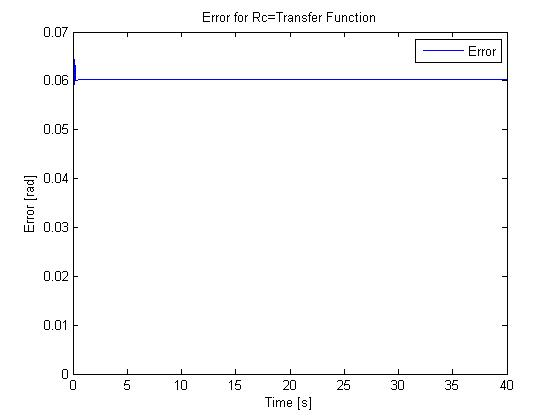
\includegraphics[width=0.9\textwidth, height = 7cm]{graphics/Ramp3Err.jpg} 
\caption{Systems error signal for a ramp input with $R_c = s$}\label{fig:Ramp3Err}
\end{figure}

\begin{figure}[htbp]%System 3 Quad
\centering
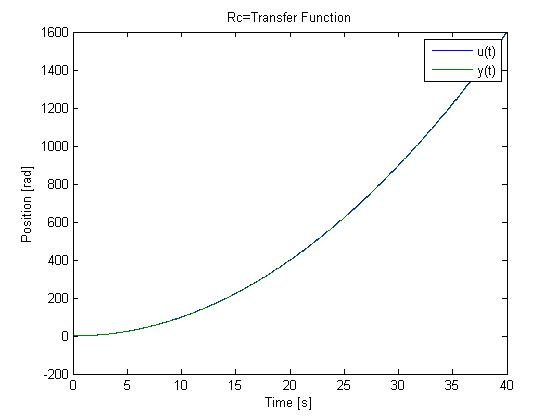
\includegraphics[width=0.9\textwidth, height = 7cm]{graphics/Quad3.jpg} 
\caption{Systems response to a quadratic input with $R_c = s$}\label{fig:Quad3}
\end{figure}

\begin{figure}[htbp]%System 3 Quad Err
\centering
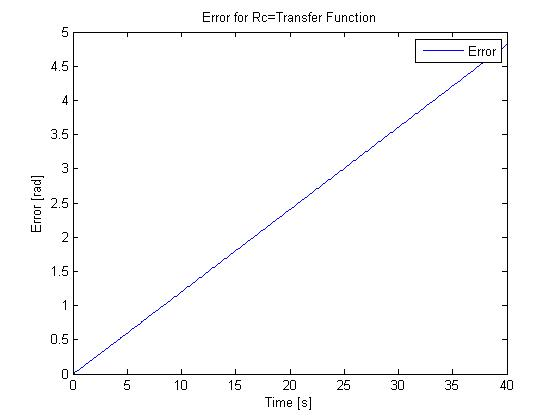
\includegraphics[width=0.9\textwidth, height = 7cm]{graphics/Quad3Err.jpg} 
\caption{Systems error signal for a quadratic input with $R_c = s$}\label{fig:Quad3Err}
\end{figure}
\end{enumerate}
\end{enumerate}
\end{document}